\subsection{Design Definition Verification}\label{sec:designVV}
The goal of design definition verification is to evaluate \progname{}'s
Module Interface Specification (MIS) for correctness, consistency,
completeness, readability, testability, and traceability. This corresponds to
the design evaluation and traceability analysis tasks in Section 9.3 of IEEE
Std 1012-2016~\citep{vvIEEE}.

\paragraph{Method} The MIS verification plan relies on peer review/document
inspection with the following stages:
\begin{enumerate}

    \item Preparation: Participants review the MIS document with respect to
    their assigned role and goals (Table~\ref{tab:rolesMIS})

    \item Meeting: Participants meet to discuss findings, potential issues,
    and proposed action plans to address them

    \item Rework: The MIS author revises the document to address raised issues,
    guided by the proposed action plans

    \item Follow Up: Participants verify that raised issues have been addressed
    satisfactorily

\end{enumerate}

A recording device might be used to capture meeting proceedings in place of
physical note taking so that all participants can focus on the discussion.

Peer review/inspection begins when there is a new major version of the MIS
document.

Peer review/inspection ends when reviewers agree that there are no issues that
will likely result in an extensive loss of confidence in \progname{} (e.g.
insufficient information hiding).

\paragraph{Roles and Responsibilities} To assist in the achievement of their
assigned goals (Table~\ref{tab:rolesMIS}) using peer review/document inspection:
\begin{itemize}

    \item Primary team members are responsible for ensuring that reviewers have
    the necessary materials, moderating the inspection process and reading
    through the document(s) during the meeting(s)

    \item Secondary and tertiary members are reviewers whom are responsible for
    reviewing the MIS document prior to the meeting so that they are prepared to
    discuss it with the team

\end{itemize}

\paragraph{Inputs}
\begin{itemize}

    \item Module Interface Specification for \progname{}: A Computational Model
    of Emotion for Enhancing Non-Player Character Believability in Games

    \item Module Guide for \progname{}: A Computational Model of Emotion for
    Enhancing Non-Player Character Believability in Games

    \item Review guide for \progname{}'s MIS
    (Appendix~\ref{appendix:designInspection})

\end{itemize}

\paragraph{Outputs}
\begin{itemize}

    \item Objective evidence to assess the verification of the MIS

    \item Objective evidence that the module design specifications are
    complete, correct, accurate, and testable

    \item Objective evidence that no unintended features were introduced into
    the design

    \item Objective evidence that the module design specifications represents a
    complete transformation of the requirements described in \progname{}'s
    Software Requirements Specification (SRS)

    \item Objective evidence that the MIS is readable

    \item Input to Master Test Report (MTR)

\end{itemize}

\paragraph{Estimated Completion Time} Four (4) weeks

Due to the number and relative complexity of the modules, MIS verification is
divided into parts by level in the use hierarchy. This ensures that modules are
verified before those that use them so that any necessary changes are made
before their verification. Only one part is tested per week to reduce
participant fatigue:
\begin{itemize}

    \item Part 1: Emotion Intensity Type (M1), Emotion Intensity Decay Rate
    Type (M5), PAD Type (M8), Social Attachment (M15), Time (M16) World State
    (M17)

    \item Part 2: Emotion State Type (M3), Goal (M12), Plan (M13), Attention
    (M14)

    \item Part 3: Emotion Intensity Decay State (M6), Emotion Decay Function
    (M7), PAD Function (M9), Emotion Type (M10)

    \item Part 4: Emotion Intensity Function (M2), Emotion Generation Function
    (M4), Emotion Function (M11)

\end{itemize}

\begin{figure}[!h]
    \centering
    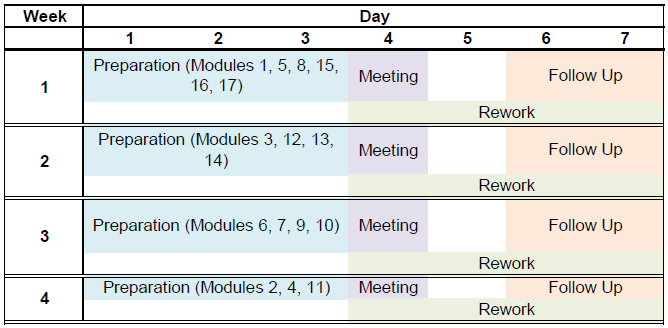
\includegraphics[width=0.9\linewidth]{figures/DesignDef_Schedule.png}
\end{figure}